\chapter{If Transformation}

\label{ch:if-transformation}

\newcommand{\opite}{\texttt{ifThenElse}}
\newcommand{\opselect}{\texttt{select}}

\section{Related work}

% Dynamic data structure -> no issues

\section{Transformation simplified}

The if construct in the Ohua framework, behaves like a curried function.
Input to the function is a boolean value and output is either the result of computing the true or the false branch.
Input values to the two conditional branches are curried from the outside.


\subsection{Splitting branches}

We can apply a very similar method of decomposition as we did with smap.
To keep the transformation simple we assume both branches to have an equal number of fetches such that always two fetches, one from each branch, can be merged together.
If we merge one fetch from each branch we know that no matter the condition, exactly one of them is going to have input present.
Hence if we select whichever input is present and feed it to our single, merged fetch it is guaranteed to have input no matter the condition.
Afterwards we will ensure the output from \fetch{} is fed back into the continuation of the branch the input came from.

A simple demonstration of this transformation in Haskell code.
Both branches consist of calculations before the fetch and after the fetch and a fetch in between, see Figure \ref{fig:if-trans-code-before}.
In order to select the present input we first bundle the before calculations into their own if construct.
This construct now returns a request for our fetch independent of the condition.
We feed the request to fetch.
We use the same condition from before to select the appropriate continuation branch and call it with the value returned from the fetch, see Figure \ref{fig:if-trans-code-after}.
As with the smap transformation this simplified model ignores the fact that not every computation can be decomposed into \texttt{after . fetch . before}, however as in smap the transformation is still correct because we are in the land of dataflow.
In practice we only close the if or smap around the fetch itself and do not touch other parts of the graph.
This way we preserve as much data independence as possible, which leads to more opportunities for Ohua to parallelise.

\begin{figure}
\begin{verbatim}
if cond
    then afterTrue  . fetch . beforeTrue
    else afterFalse . fetch . beforeFalse
\end{verbatim}
\caption{Code before transform}
\label{fig:if-trans-code-before}
\begin{verbatim}
(if cond
     then afterTrue
     else afterFalse)
. fetch
. (if cond
       then beforeTrue
       else beforeFalse)
\end{verbatim}
\caption{Code after transform}
\label{fig:if-trans-code-after}
\end{figure}

\subsection{Fetch imbalance}

We previously assumed that both branches held an equal number of fetches and that these could be paired up neatly in twos.
However in real programs this may not be the case at all, see Figure \ref{fig:if-trans-code-uneq-before}.
There is a simple solution to this problem.
We solve the imbalance of fetches by inserting empty (NoOp) fetches at the front of the branch with fewer fetches, see Figure \ref{fig:if-trans-code-uneq-inserted}.

\begin{figure}
\begin{verbatim}
if cond
    then afterTrue . fetch . beforeTrue
    else falseBranch
\end{verbatim}
\caption{Code with unequal number of fetches}
\label{fig:if-trans-code-uneq-before}
\begin{verbatim}
if cond
    then afterTrue         . fetch . beforeTrue
    else const falseBranch . fetch . mkEmptyRequest
\end{verbatim}
%(if cond then afterTrue else const falseBranch) . fetch . (if cond then beforeTrue else mkEmptyRequest)
\caption{Inserting an empty fetch}
\label{fig:if-trans-code-uneq-inserted}
\begin{verbatim}
(if cond
     then afterTrue
     else const falseBranch)
. fetch
. (if cond
       then beforeTrue
       else mkEmptyRequest)
\end{verbatim}
\caption{Transformed code with unequal number of fetches}
\label{fig:if-trans-code-uneq-after}
\end{figure}

Originally I would create the empty fetches by collecting an ordered list of fetches on each branch.
They would be ordered by dependency, hence the first one would depend on no other fetch in the sequence, the second one would only depend on the first one, the third one on either two and so on.
After that I would calculate the difference in length between both lists to obtain a number of necessary empty fetches.
Then I would generate a sequence of request-fetch pairs as long as the calculated difference.
These would then be connected in sequence.
The first one would receive input from the last fetch of the shorter of the two previously calculated sequences of preexisting fetches.
Since these are NoOp they ignore their inputs, we use the inputs only to create data dependencies.
If the shorter sequence of preexisting fetches was empty a new operator \texttt{null} would be created and inserted.
This operator would not get input at all, except for a context arc from the \texttt{if} and emit a data packet containing \texttt{null} used to activating the first created fetch.
The second request-fetch pair would receive as input the result from the first fetch and the third one the result from the second and so on.
The final result was discarded

There is a significant problem with this approach, which is, and I only realised this late, that this created sequence is fully dependent.
Meaning each fetch depends on \textbf{all} of its predecessor fetches.
We have created a branch which contains a sequence of fully dependent fetches.
However there is no erason why the other, longer branch should be fully dependent also.
The result is that, once we merge both branches around the fetches the resulting combined fetches inherit both data dependencies.
Since you cannot depend on more than literally all predecessors the resulting merge inherits its dependence from the fully dependent second branch.
In the the second branch each fetch was dependent on all previous fetches in the branch, and from this follows that it will have to be in a separate fetch round to all its predecessors.
And since this is true for all fetches in the branch each of those will be in a separate round.
They can still be batched with other, parallel parts of the program, however we have lost the opportunity for some batching here, because we have forced sequentiality, even if it may not have existed originally.

There is a very simple solution to this problem, which, coincidentally, also simplified the implementation of the algorithm as a whole.
Now I always generate a \texttt{null} operator with no dependency other than the \texttt{if}, a single NoOp request creating operator, the output of which is fed into a number of generated fetches.
Therefore we only create one request, which reduces the number of operators, and the fetches depend only on the \texttt{if} operator.
Therefore they could in theory all be batched.
If we now merge the branches our empty requests will create no new dependencies, since they have the least dependency possible in the branch.

The observant reader will have noticed this only solves the problems for empty requests but does not take into account how the preexisting fetches on those branches may differ in dependencies and may influence and delay each other when merging.
This will be subject of future improvements where we aim to increase efficiency my separately batching subgraphs of the program and this, we hope, should lead to an optimal result in that case as well.

Now we can apply the transformation as we did before, see Figure \ref{fig:if-trans-code-uneq-after}.

\section{Transformation in operators}

More concretely \texttt{if} is composed of a starting node called \opite{} and an end node called \opselect{}, see Figure \ref{fig:basic-if}.
The \opite{} operator takes as its input the boolean value and depending on the value activates one of its two outputs.
Outputs from the \opite{} operator are connected via an activation arc to the first operator(s) of each of the respective conditional branches.
The computed output from the conditional branches are both fed to the \opselect{} operator which returns a value whenever one of its inputs receives one.

\begin{figure}
	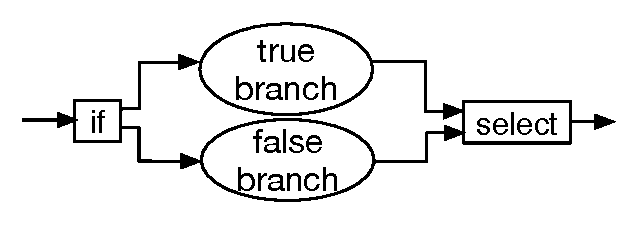
\includegraphics[width=\textwidth]{Figures/basic-if}
	\caption{Dataflow representation of if}
	\label{fig:basic-if}
\end{figure}

To close out our fetch from the if we replace the original two fetches with a select operator, receiving both their inputs and feeding into a single fetch.
The output from this fetch is fed back to \textbf{both} continuation branches.
Any location that used either fetch result now receives the result of the combined fetch.
This might seem wrong, however we use a new \opite{} to only select one of the two branches for execution, therefore only the originally selected branch also continues with its execution.

\begin{figure}
	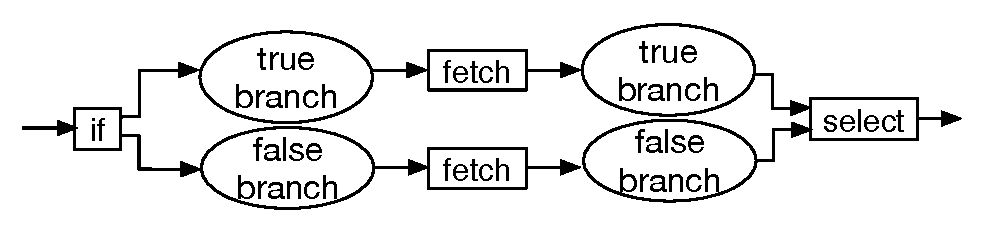
\includegraphics[width=\textwidth]{Figures/basic-if-rewrite-original}
	\caption{If rewrite source graph}
	\label{fig:if-rewrite-graph-before}
	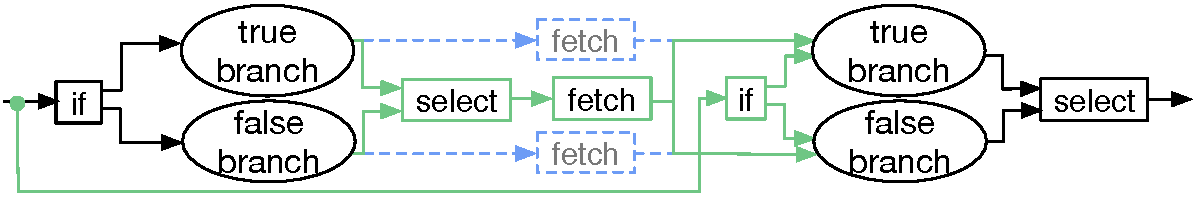
\includegraphics[width=\textwidth]{Figures/basic-if-rewrite}
	\caption{If rewrite transformed graph}
	\label{fig:if-rewrite-graph-after}
\end{figure}
